% CREATED BY DAVID FRISK, 2016
% MODIFIED BY JAKOB JARMAR, 2016
% A few changes by Birgit Grohe, 2017 and 2018
% Adjustments with the help of Gustav Örtenberg 2019
% Parskip % bibliography system updated by Erik Ljungdahl, May 2022

% IMPORT SETTINGS
\documentclass[12pt,a4paper,twoside,openright]{report}
% CREATED BY LEVENTE VARGA, 2024

% BASIC SETTINGS
\usepackage{moreverb}								% List settings
\usepackage{textcomp}								% Fonts, symbols etc.
\usepackage{lmodern}								% Latin modern font
\usepackage{helvet}									% Enables font switching
\usepackage[T1]{fontenc}							% Output settings
\usepackage[english]{babel}							% Language settings
\usepackage[utf8]{inputenc}							% Input settings
\usepackage{amsmath}								% Mathematical expressions (American Mathematical Society)
\usepackage{amssymb}								% Mathematical symbols (American Mathematical Society)
\usepackage{graphicx}
\graphicspath{images/}
    % Figures
\usepackage{subfig}									% Enables subfigures
\numberwithin{equation}{chapter}					% Numbering order for equations
\numberwithin{figure}{chapter}						% Numbering order for figures
\numberwithin{table}{chapter}						% Numbering order for tables
\usepackage{minted}						    		% Enables source code listings
\usepackage{chemfig}								% Chemical structures
\usepackage[top=3cm, bottom=3cm,
			inner=3cm, outer=3cm]{geometry}			% Page margin lengths			
\usepackage{eso-pic}								% Create cover page background
\newcommand{\backgroundpic}[3]{
	\put(#1,#2){
	\parbox[b][\paperheight]{\paperwidth}{
	\centering
	\includegraphics[width=\paperwidth,height=\paperheight,keepaspectratio]{#3}}}}
\usepackage{float} 									% Enables object position enforcement using [H]
\usepackage{parskip}								% Enables vertical spaces correctly 
\usepackage{datetime2} % date formatting tools - ISO-date YYYY-MM-DD
\usepackage{microtype} % Microtypography - improves readability and appearance of text.

% Allows clickable links for references, in table of contents, autoref, etc.  	
\usepackage{hyperref}								
\hypersetup{colorlinks, citecolor=black,
   		 	filecolor=black, linkcolor=black,
    		urlcolor=black}

%% Bibliography https://www.overleaf.com/learn/latex/Bibliography_management_with_biblatex
\usepackage[style=ieee]{biblatex} % style=apa also possible
\addbibresource{references.bib}


% OPTIONAL SETTINGS (DELETE OR COMMENT TO SUPPRESS)
		 

% Define the number of section levels to be included in the t.o.c. and numbered	(3 is default)	
\setcounter{tocdepth}{5}							
\setcounter{secnumdepth}{5}	


% Chapter title settings
\usepackage{titlesec}		
\titleformat{\chapter}[display]
  {\Huge\bfseries\filcenter}
  {{\fontsize{50pt}{1em}\vspace{-4.2ex}\selectfont \textnormal{\thechapter}}}{1ex}{}[]


% Header and footer settings (Select TWOSIDE or ONESIDE layout below)
\usepackage{fancyhdr}								
\pagestyle{fancy}  
\renewcommand{\chaptermark}[1]{\markboth{\thechapter.\space#1}{}} 


% Select one-sided (1) or two-sided (2) page numbering
\def\layout{2}	% Choose 1 for a one-sided or 2 for a two-sided layout
% Conditional expression based on the layout choice
\ifnum\layout=2	% Two-sided
    \fancyhf{}			 						
	\fancyhead[LE,RO]{\nouppercase{ \leftmark}}
	\fancyfoot[LE,RO]{\thepage}
	\fancypagestyle{plain}{			% Redefine the plain page style
	\fancyhf{}
	\renewcommand{\headrulewidth}{0pt} 		
	\fancyfoot[LE,RO]{\thepage}}	
\else			% One-sided  	
  	\fancyhf{}					
	\fancyhead[C]{\nouppercase{ \leftmark}}
	\fancyfoot[C]{\thepage}
\fi


% Inline code snippets from: https://tex.stackexchange.com/questions/661993/recreate-markdown-style-inline-code-blocks-in-latex
\usepackage{tikz}
\tikzset{%
    baseline,
    inner sep=2pt,
    minimum height=12pt,
    rounded corners=3pt  
}
\newcommand{\code}[1]{\mbox{
    \ttfamily
    \tikz \node[anchor=base,fill=black!4]{#1};
}}


% Enable To-do notes
\usepackage[textsize=tiny]{todonotes}   % Include the option "disable" to hide all notes
\setlength{\marginparwidth}{2.5cm} 


% Suppress warning from Texmaker about head-height
\setlength{\headheight}{15pt}		





\newcommand{\oneLineTitle}{Video Game Genre Blending (Working Title)}
\newcommand{\multiLineTitle}[1]{Video Game Genre Blending \\[#1] (Working Title)}
\newcommand{\researchQuestionOne}{\textit{Which genres of games can be extracted and combined to create a new game type?}}
\newcommand{\researchQuestionTwo}{\textit{What implications can be derived by implementing a game based on a combination of specific game genres?}}
% The term [#1] indicates that there will be 1 break to split the title into two pieces, the first part before \\[#1] and the second part after. If you have a very long title and need to split it up into 3 rows, just use \\[#1] multiple times.

\newcommand{\oneLineSubtitle}{}
\newcommand{\authorName}{Levente Varga}


\begin{document} 


% COVER PAGE, TITLE PAGE AND IMPRINT PAGE
\pagenumbering{roman}			% Roman numbering (starting with 'i' (one)) until the first main chapter
% CREATED BY DAVID FRISK, 2016
% MODIFIED BY JAKOB JARMAR, 2016
% A few changes by Birgit Grohe, 2017 and \the\year
% Adjustments with the help of Gustav Örtenberg 2019

% COVER PAGE
{ %% Scoped to not change parskip outside the titlepage


\begin{titlepage}
\newgeometry{top=3cm, bottom=3cm,
			left=2.25 cm, right=2.25cm}	% Temporarily change margins		
			
% Cover page background 
\AddToShipoutPicture*{\backgroundpic{-4}{56.7}{figure/auxiliary/frontpage_gu_eng_vec_m2.pdf}}
\addtolength{\voffset}{2cm}

% Cover picture (replace with your own or delete)		
\begin{figure}[H]
\centering
\vspace{1cm}	% Adjust vertical spacing here
%\includegraphics[width=0.9\linewidth]{figure/somepicture}
\end{figure}

% Cover text
\mbox{}
\vfill
\renewcommand{\familydefault}{\sfdefault} \normalfont % Set cover page font

\textbf{\Huge \multiLineTitle{0.2cm}} 
\\[0.5cm]

% {\Large \oneLineSubtitle}\\[0.5cm]

%{\Large A Subtitle that can be Very Much Longer if Necessary}\\[0.5cm]

Master's thesis in Computer science and engineering \setlength{\parskip}{1cm}

{\Large \authorName} \setlength{\parskip}{2.9cm}

Department of Computer Science and Engineering \\
\textsc{Chalmers University of Technology} \\
\textsc{University of Gothenburg} \\
Gothenburg, Sweden \the\year

\renewcommand{\familydefault}{\rmdefault} \normalfont % Reset standard font
\end{titlepage}


% BACK OF COVER PAGE (BLANK PAGE)
\newpage
\restoregeometry
\thispagestyle{empty}
\mbox{}


% TITLE PAGE
\newpage
\thispagestyle{empty}
\begin{center}
	\textsc{\large Master's thesis \the\year}\\[4cm]		% Report number is currently not in use
	\textbf{\Large \multiLineTitle{0.2cm}} \\[1cm]
        % {\large \oneLineSubtitle}\\[1cm]
	{\large Levente Varga}
	
	\vfill	
	% Logotype on the title page	
	\begin{figure}[H]
	\centering
	% Remove the following line to remove the title page logotype
	
\includegraphics[width=0.25\pdfpagewidth]{figure/auxiliary/ChGULogoHog.pdf}
	\end{figure}	\vspace{5mm}	
	
	Department of Computer Science and Engineering\\
	%\emph{Division of Division name}\\
	%Name of research group (if applicable)\\
	\textsc{Chalmers University of Technology} \\
	\textsc{University of Gothenburg} \\
	Gothenburg, Sweden \the\year \\
\end{center}


% IMPRINT PAGE (BACK OF TITLE PAGE)
\newpage
\thispagestyle{plain}
\vspace*{4.5cm}
\oneLineTitle\\
\oneLineSubtitle\\
\authorName \setlength{\parskip}{1cm}

\copyright ~ \authorName, \the\year. \setlength{\parskip}{1cm}

Supervisor: Natasha Bianca Mangan, Department of Computer Science and Engineering\\
Examiner: Name, Department \setlength{\parskip}{1cm}

Master's Thesis \the\year\\	% Report number currently not in use 
Department of Computer Science and Engineering\\
%Division of Division name\\
%Name of research group (if applicable)\\
Chalmers University of Technology and University of Gothenburg\\
SE-412 96 Gothenburg\\
Telephone +46 31 772 1000 \setlength{\parskip}{0.5cm}

\vfill
% Caption for cover page figure if used, possibly with references to further information in the report
Cover: Description of the picture on the cover page (if applicable)


Typeset in \LaTeX \\
%Printed by [Name of printing company]\\
Gothenburg, Sweden \the\year

}

% ABSTRACT
\newpage
% CREATED BY DAVID FRISK, 2016
\oneLineTitle\\
\oneLineSubtitle\\
\authorName\\
Department of Computer Science and Engineering\\
Chalmers University of Technology and University of Gothenburg

\thispagestyle{plain}			% Suppress header 
\section*{Abstract}
Abstract text about your project in  Computer Science and Engineering.

% KEYWORDS (MAXIMUM 10 WORDS)
\vfill
Keywords: Computer science, video game.

\newpage				% Create an empty back of side
\thispagestyle{empty}
\mbox{}

% ACKNOWLEDGEMENTS
%\newpage
%% CREATED BY DAVID FRISK, 2016
\thispagestyle{plain}			% Suppress header
\section*{Acknowledgements}
Here, you can say thank you to your supervisor(s), company advisors and other people who supported you during your project.

\vspace{1.5cm}
\hfill
\authorName, Gothenburg, \today

\newpage				% Create an empty back of the side
\thispagestyle{empty}
\mbox{}


% TABLE OF CONTENTS
\newpage
\tableofcontents

% OTHER FRONTMATTER
% List of figures (add to table of contents)
\cleardoublepage
\phantomsection
\addcontentsline{toc}{chapter}{\listfigurename} 
\listoffigures
% List of tables (add to table of contents)
\cleardoublepage
\phantomsection
\addcontentsline{toc}{chapter}{\listtablename}
\listoftables


% START OF MAIN DOCUMENT
\cleardoublepage
\setcounter{page}{1}
\pagenumbering{arabic}			% Arabic numbering starting from 1 (one)

\chapter{Introduction} \label{Chapter:Introduction}

% TODO: Look at other papers to see how they structure Introduction, Methods and Background

% Most similar paper: \cite{ljungdahl2020individual}

\section{Background}

In the second half of the twentieth century, often referred to as the dawn of the digital age or the prehistory of the computer game\cite{malliet2005history}, video games started to emerge as a new leading medium. Unlike today's blockbusters, which are often the result of the collaboration between multiple international studios, early video games were typically developed by just a handful of people and featured limited and basic gameplay elements and mechanics. 

Over time, genre boundaries began to blur, while entirely new genres started to form. At the same time, the gaming industry has undergone a rapid evolution in both production scale, quantity, and variety, and introduced new hybrid game genres through a process known as genre blending\cite{arsenault2009}, which combines key concepts from existing genres. This process has led to increasing commercial success, as genre-blended games usually stand out with their unique mix of game mechanics and diverse gameplay, appealing to a broader audience.



\subsection{A brief history of video games}

It is challenging to tell exactly when the video game era began, as there is ongoing debate over what constitutes the first video game. Some consider it to be Tennis for Two (1958)\cite{tennisfortwo1958}, an abstract 2D simulation of tennis played on an oscilloscope. However, its creator, Willy Higinbotham, developed it solely to demonstrate the capabilities of the hardware it was running on. As a result, there was no scoring system, nor any other feature that would resemble a modern video game\cite{malliet2005history}.

A stronger candidate for being the first true video game is Spacewar (1962) \cite{spacewar1962}, developed by Steve Russell during his time in college. Unlike Tennis for Two, Spacewar was intended to be a way of entertainment for two players. It was programmed on PDP-1 mainframe computers and featured a simplified representation of space with two controllable spaceships, a black hole located in the middle of the screen, and a few blinking stars for decoration. Players competed to destroy each other's spaceship using torpedoes while avoiding crashing into the black hole. Since Spacewar was a computer program intentionally developed for entertainment, it is widely regarded as the first true video game. Furthermore, it laid the groundwork for the action and simulation genres that emerged shortly after\cite{malliet2005history}.

Interestingly, most people would mistakenly believe that the first video game was Pong\cite{pong1972}, probably due to its massive popularity. However, it was released a full decade after Spacewar, in 1972.



\subsection{Genre combinations}

In 1993, Doom\cite{doom1993} was released, a prime example of a genre being born. Even though Doom was not the first of its kind, and just like other games, it was a combination of already existing game types like action and shooter, it became so successful and popular that the common term to describe similar games became "doom-clone". Only a couple of years later did a proper name "first-person shooter" (FPS) for these types of games appear and gain mass acceptance\cite{arsenault2009}, thus giving birth to a new video game genre.

Soulslike games share a similar story, although 'Soulslike' is not considered a genre of its own, but rather a subgenre. Its name comes from games developed by FromSoftware, a game development studio which is mainly famous for its games of high difficulty, namely Demon's Souls and the Dark Souls trilogy, all built around a very similar theme and game aesthetics, dynamics and mechanics\cite{hunicke2004mda}. Since these games are relatively new (the oldest of them, Demon's Souls, was released in 2009), a better and more descriptive name for this sub-genre has not been found yet.



\section{Thesis}



\subsection{Motivation}

Although numerous genre combinations already exist, there are still many unexplored possibilities that could lead to the creation of engaging and innovative games. By examining existing combinations and identifying gaps in the market, this research aims to propose new genre fusions that could offer new gameplay experiences. The ultimate goal is to develop a game based on one of these novel combinations.

Due to the limited time available for the thesis, the development of a complete game is unlikely. Instead, the feasibility of the proposed genre blend will be demonstrated by a game prototype that will retain all the characteristics and core concepts of each chosen genre, with limited visual appeal and polish. More about limitations will be discussed in section \ref{Section:Limitations}.



\subsection{Research questions}

The core motivation driving this research is to find out whether it is feasible to blend elements of a specific genre combination into a single, functional gameplay experience that has not been done before. The first part of this study is to discover these combinations and analyze their feasibility, then, as the second part, test it using a game prototype and gain feedback from playtesting sessions to examine the practical implications and player perceptions of such a hybrid game.

The following research questions will guide this research.

\textbf{RQ1:} \researchQuestionOne

The first part of the thesis will answer RQ1, first observing what game types exist already, then coming up with new ones, and finally, a genre combination will be chosen to be implemented into a game prototype to help answer RQ2, which is:

\textbf{RQ2:} \researchQuestionTwo

Since RQ1 serves as the base for the development of the game prototype, it must be answered earlier than RQ2. For that, chapter \ref{Chapter:Planning} was introduced. Thus, chapter \ref{Chapter:Implementation} will only present the implementation of the game prototype.  



\subsection{Goals and Challenges}

The main goal is to come up with a new video game genre combination, and develop a functional game prototype that successfully combines all the elements and mechanics of the selected genres. Even if the resulting gaming experience turns out to be unenjoyable, it could still serve as a valuable lesson and a good indicator that these genres might not fit well together.

The core challenge - as with most games - is to achieve player satisfaction. Players who become frustrated and do not enjoy playing the game could indicate a potential design flaw and the wrong combination of genres. It could also mean that not the right players were selected for testing, therefore it is crucial to conduct a brief 'pre-screening' of playtesters to ensure that the potential target audience are the ones testing the game. This is in an attempt to avoid unnecessary dissatisfaction and thus unwanted outliers in the feedback data.



\subsection{Limitations} \label{Section:Limitations}

To allow more time for the development of the prototype, the research was affected by the following limitations:

\begin{itemize}
    \item An existing data set of games was used, which was not up-to-date. Getting the most recent data would have taken significant extra work while providing minimal impact on the result.
    \item Given the vast amount of possible combinations of video game genres, the complete list was not discussed. Instead, a few promising genres were pre-selected and tested to see if their combinations exist.
    \item Steam tags were used to find existing genre combinations. Although tags do not necessarily represent genres, Steam has an extensive database of its library, and tags are the most useful way of categorization found during research, making them a viable choice.
\end{itemize}

The game prototype was struck by the following limitations due to the limited amount of time:

\begin{itemize}
    \item The graphics, audio and other assets used were primitive to save time.
    \item The focus was on developing the core gameplay, instead of decorative features like a detailed settings page, achievements, or advanced accessibility features.
    \item The prototype was only developed for Windows, without any planned support for other platforms.
    \item The game only supports the 16:9 aspect ratio, since this is the most popular. Taking care of other aspect ratios would have been a waste of time regarding the goal of the thesis.
    \item There is no tutorial or any proper introduction to the game and its mechanics, since during playtests, players were given guidance when it seemed necessary.

    % TODO: Add more as the prototype progresses
    
\end{itemize}
\chapter{Theory} \label{Chapter:Theory}

This chapter is about the literature review that will serve as a valuable background for future research.



\section{Defining video game genres}

The first attempts to classify video games occurred years after the first video game was released. In his book published in 1984, Chris Crawford listed games in two major categories, namely skill and action games (S\&A) which rely heavily on hand-eye coordination and motor skills and are usually fast-paced, and strategy games that emphasize more decision-making, and due to their nature, they generally take longer than S\&A games\cite{crawford1984art}. Within these main categories, Crawford defined multiple subdivisions for finer categorization. Some of these categories have evolved into modern game genres and are still present today, like sports and adventure games, while others, including paddle games, D\&D games and games of chance have completely merged into other genres and do not exist on their own. It is important to note that Crawford did not refer to these categories as genres.

Many of the first definitions of true video game genres were formulated by Mark J. P. Wolf, who also compared video games with the other existing media types, but mainly cinema \cite{wolf2002genre}. He concluded that video games and movies, while many similarities exist, can not be categorized the same way, due to their differences in interactivity (video games require active participation from the audience). Thus, the 41 genres and subgenres explained in his paper\cite{wolf2002genre} are based on interactivity aspects, instead of iconography. The border between some of these genres is blurry, Racing and Driving, Catching and Capturing, Obstacle Course, and Platform all have a surprisingly similar definition to the other, differing only in a few parameters; however, these similarities are explicitly stated by the author.

Another approach was made in 2006 by Thomas H. Apperley, who agreed with Wolf that games cannot be categorized like other media types. He also criticized earlier game categorization attempts, mainly because they are "loose aesthetic clusters based around video games' aesthetic linkages to prior media forms"\cite{apperley2006genre}. Instead, his proposed framework tries to shape a new set of genres around the style of "ergodic interaction" that takes place within the games. In his paper, he defined four distinct video game genres. \textit{Simulation} games mimic the intricate processes of real-life systems, such as cars or cities. \textit{Strategy} games, including real-time strategy (RTS) and turn-based strategy (TBS), are outliers due to their similarity to board games. These games usually have a god's-eye view and information-heavy interfaces. \textit{Action} games include first-person shooters (FPS) and third-person games and focus more on the player's performance in combat manoeuvres and aiming with weapons, and unlike strategy games, they do not contain complex decision-making processes. And finally, \textit{role-playing} games (RPG), often compared to pencil-and-paper RPGs such as Dungeons and Dragons, usually revolve around fantasy themes and focus on some form of character development, such as the collection of experience or skill points.

The early video game taxonomies were not applicable to the modern genres that followed\cite{starosta2024tangled}. Such complex genres as Massively Multiplayer Online Role-Playing Games (MMORPG) or Multiplayer Online Battle Arenas (MOBA) could not fit into the existing categories that were shaped, as they are a mix of several already defined game types (Multiplayer and Role-Playing).

Overall, it can be observed that the video game industry is and has always been struggling to come up with a universal organization system for games. Existing categorization methods, such as those used for books or movies, could not be applied due to differences between the mediums\cite{lee2014facet}.

Instead of sticking to one taxonomy, Steam\cite{steam}, an online video game store, uses a list of predefined, as well as user-defined tags (consisting of one or a few words) to categorize games published on the platform. Tags are similar, and sometimes identical, to the name of genres discussed in the above-mentioned papers, however, there is no definition linked to them. What each tag means is determined by the types of games assigned to them on the platform. This enables greater freedom in video game categorization than sicking to a chosen taxonomy would, since tags can expand and adapt to new game types, while taxonomies remain the same.



\section{Finding genre combinations}

Today's most popular game store on PC, Steam\cite{steam}, which, at the time of writing, has a library of over 204.000 apps, including the majority of modern video games. There are some exceptions, however, as some games are platform-specific and thus have never been released on Steam, but the number of such games can only be measured in the hundreds, so they will be considered insignificant for this research.

Steam uses two systems to categorize this massive amount of content. First, developers and publishers pick from a list of pre-defined genres to assign to their apps during upload. Second, users who download these apps can assign them user-defined tags that can indicate genre, theme, aesthetics, or even difficulty, and help other users find new apps that are to their liking. From the user's point of view, only the tags are visible on the apps' dedicated pages while genres are only used as filtering in the store's search field.

Steam has a public API (Application Programming Interface) that can be used to query data about their games and apps. This API, however, is not well-documented, thus it would take a considerable amount of trial and error to use it properly. Luckily, a relatively fresh dataset\cite{steamCatalogInsight2024} can be found on GitHub that, according to the author, was acquired in October 2024 using the Steam API and contains all the data necessary to find existing genre combinations on Steam. To check exactly how up-to-date this data set is, I checked the number of games under some tags on Steam and compared them with the numbers found in the data set, and the differences were around 40\%, which is unexpectedly high. However, games released in October 2024 can be found in the data set as expected with the correct release dates, indicating the data was truly acquired in or after October 2024. The explanation for such a large difference in the numbers could be explained by the ever-rising number of new games published each month on the platform and the new tags applied to games during this two-month period. However, the ratio between the tag occurrences could not change significantly in such a short time. These data are in CSV format which is mostly used by spreadsheet editors such as Excel or Numbers, but can easily be read from script too.

Going through the data set and individually counting the times each tag occurs, it is easy to determine that Steam currently uses 447 tags and 121 genres. It can also be observed that tag occurrences, as seen in figure \ref{figure:tags}, like many other data sets, seem to follow Zipf's law loosely\cite{li2002zipf}. Interestingly, some of the tags make little sense, like "Intentionally Awkward Controls" or "TrackIR", and do not represent a genre, but rather some other aspect of the game. There are a few tags like "Warhammer 40K" that solely indicate which franchise the game belongs to.

\begin{figure}[h]
    \centering
    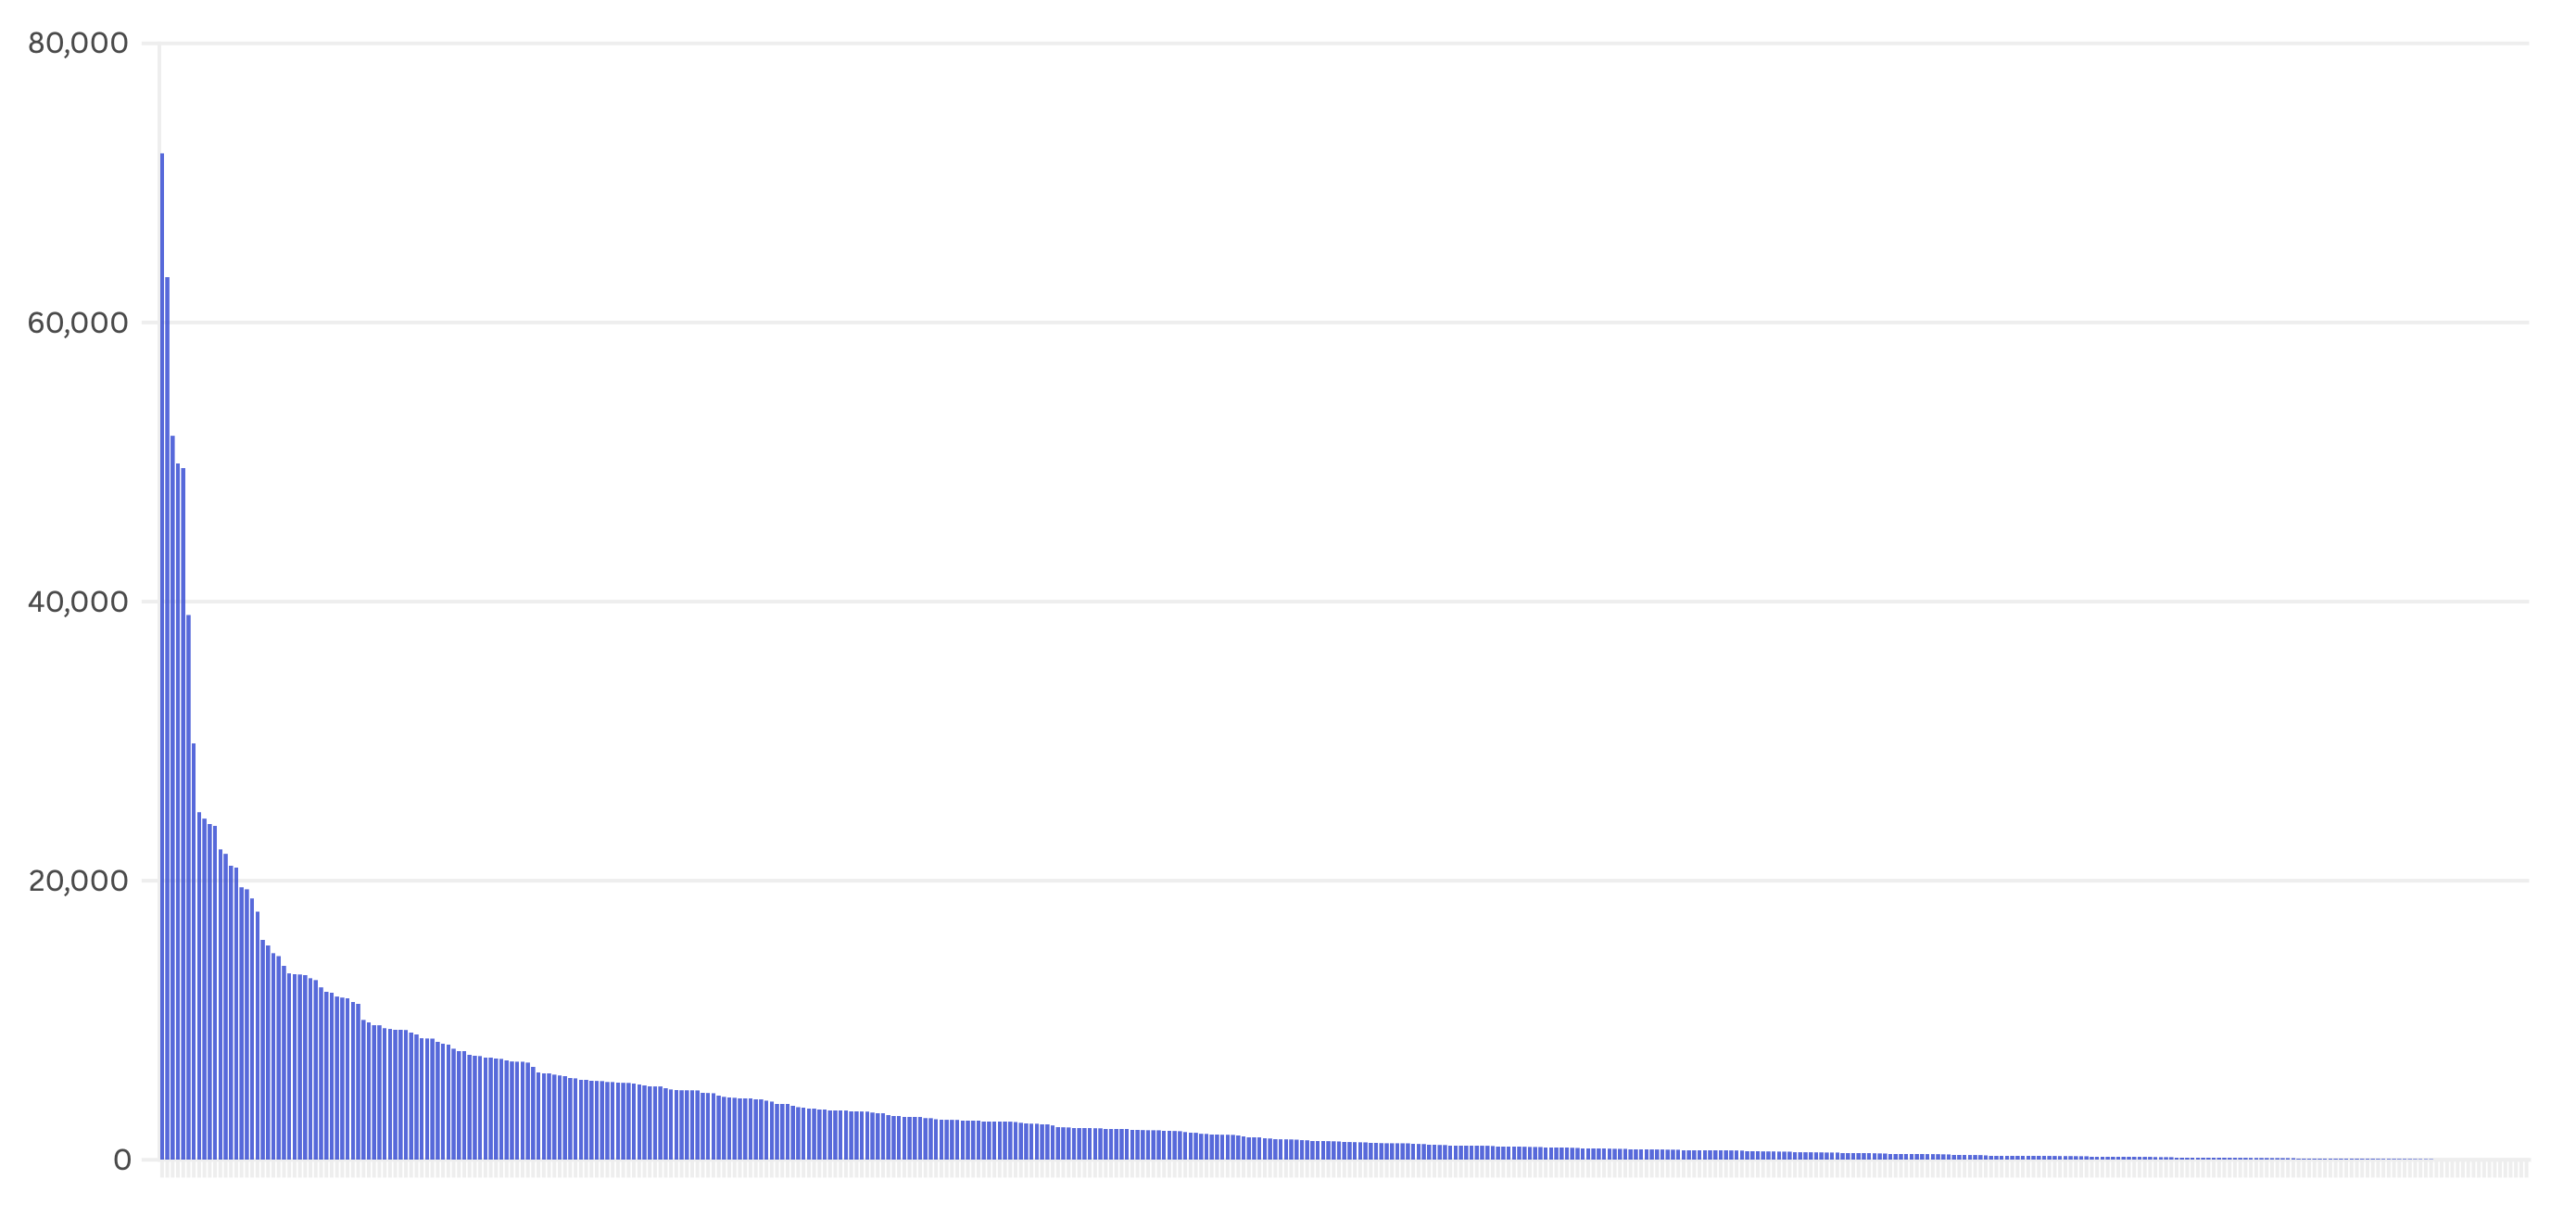
\includegraphics[width=\textwidth]{images/tag-occurrences.png}
    \caption{Tag occurrences}
    \label{figure:tags}
\end{figure}

On the other hand, the genre distribution in figure \ref{figure:genres} seems unbalanced. The reason for that is that for some reason, 84 of the 121 genres are localized versions of others, and each appears less than 30 times. These genres can be safely discarded, as their occurrence times would not contribute too much to the other numbers.

\begin{figure}[h]
    \centering
    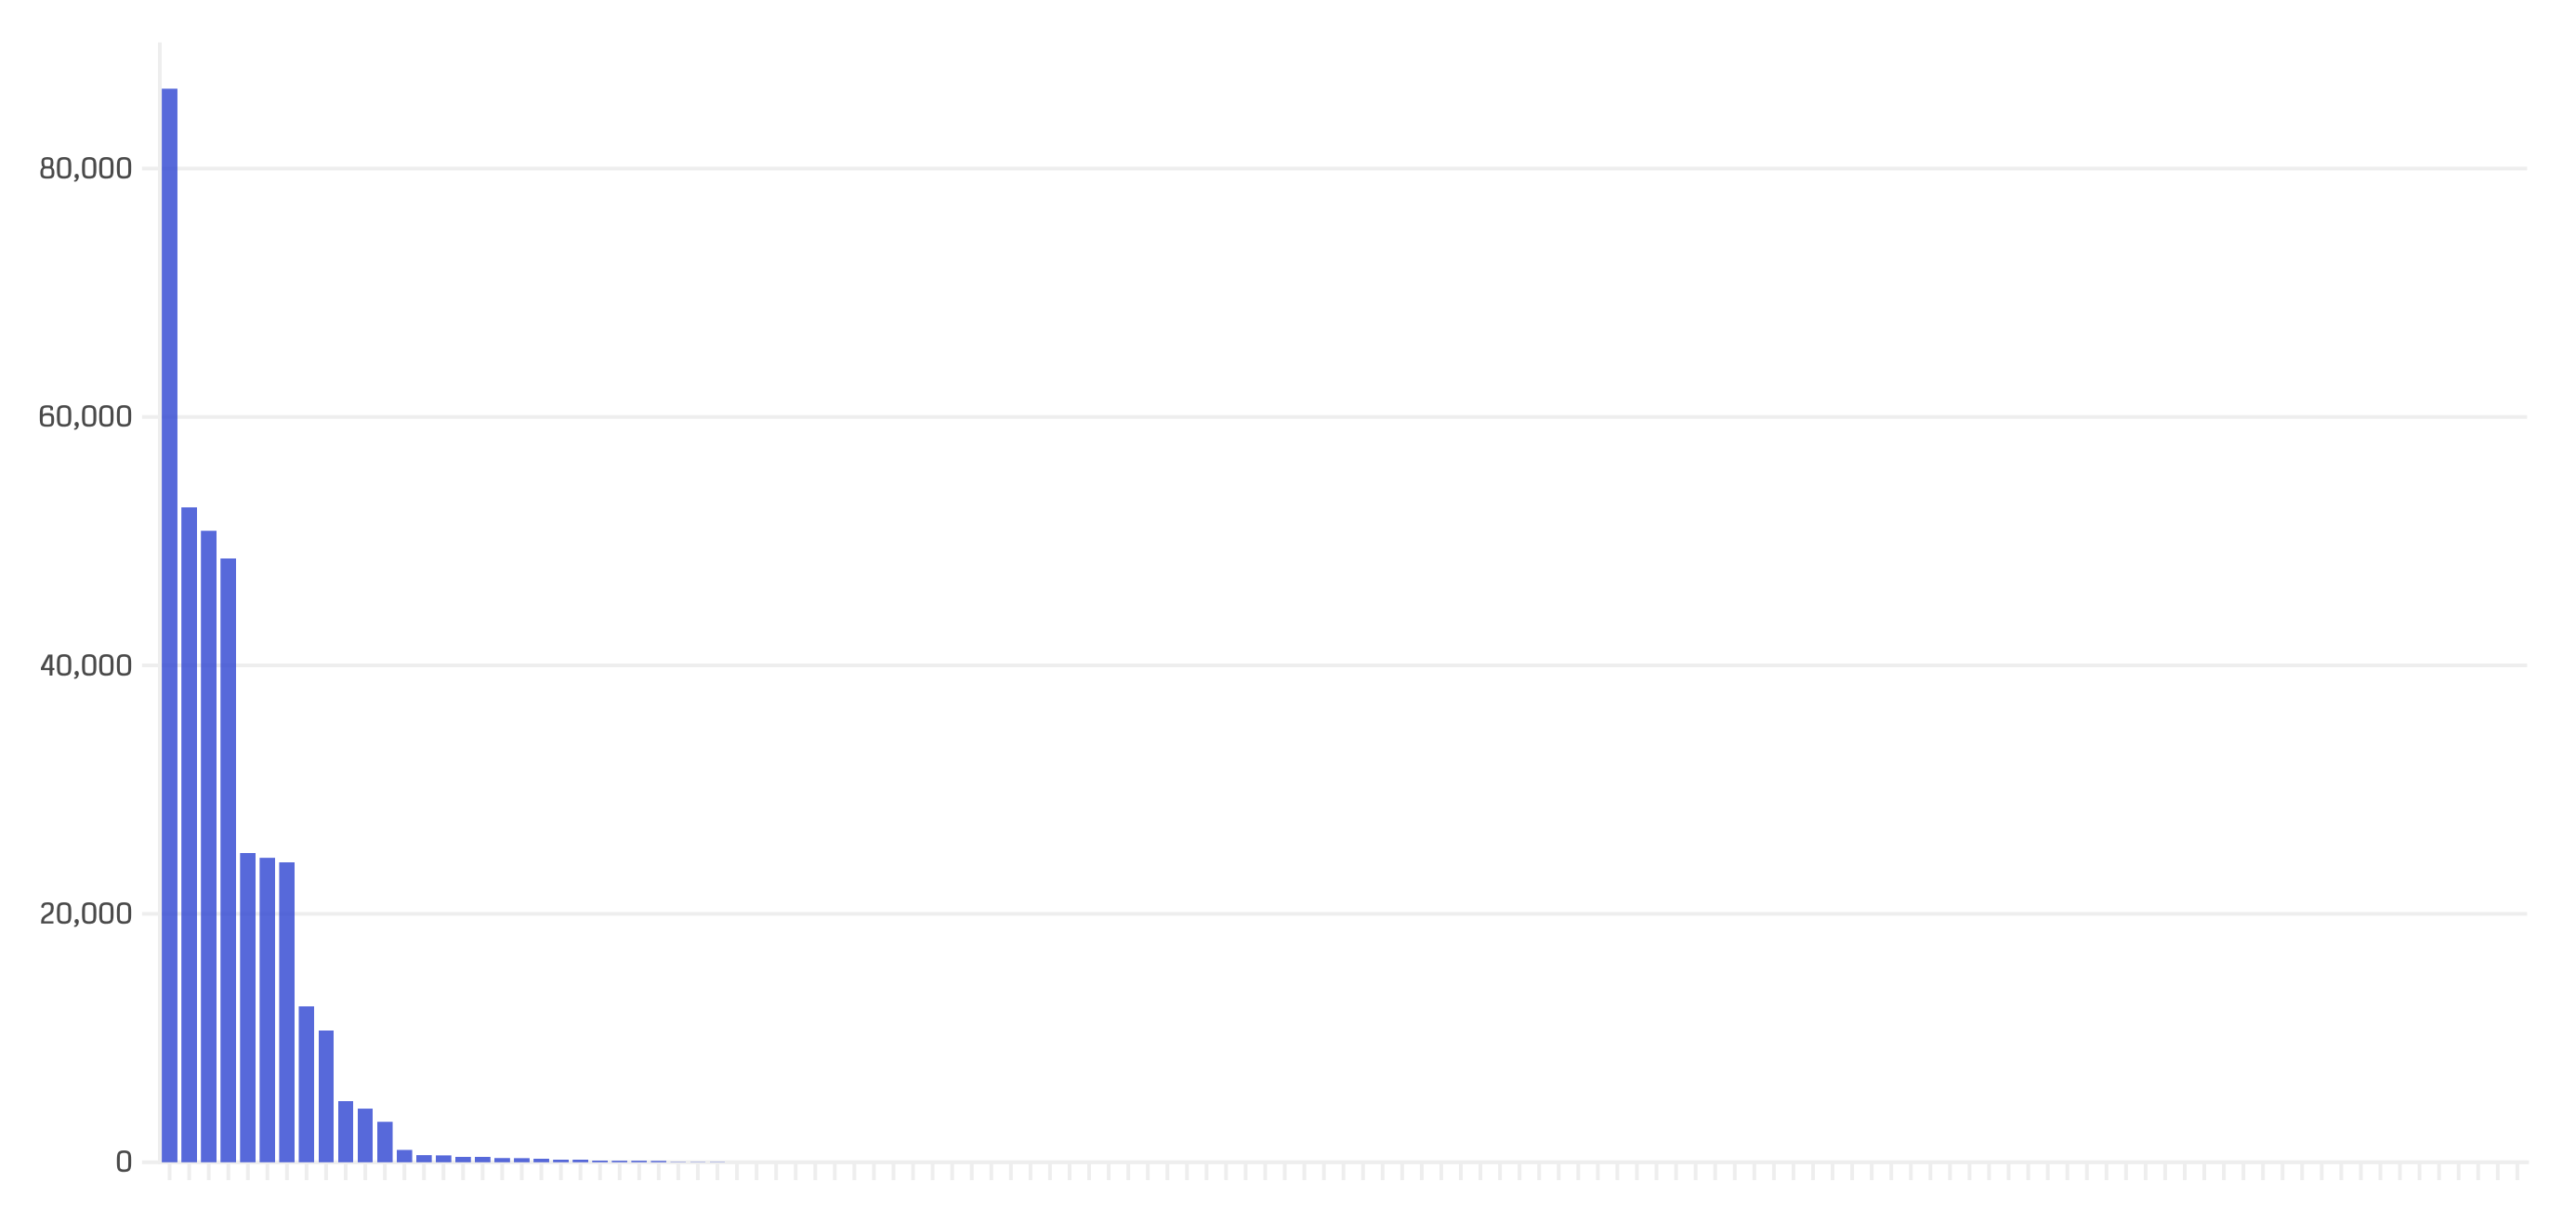
\includegraphics[width=\textwidth]{images/genre-occurrences.png}
    \caption{Genre occurrences}
    \label{figure:genres}
\end{figure}

However, since Steam uses only a handful of genres to categorize games, these genres are vague. Therefore, for this thesis, I will use Steam tags instead, as tags provide a much finer way to describe what genres the developed game prototype should belong to and what types of game mechanics they use.

It is important to note that the dataset's author also looked for genre combinations as seen in figure \ref{figure:genre-pairs}, but they only used combinations of two genres, while I was more interested in more complex mixtures. Furthermore, they only included tags assigned to at least 900 games in the Steam library, and that criteria takes away almost half of the tags. For this thesis, I was interested in the other half of the tags, those that are used rarely but at the same time clearly represent a genre or sub-genre. To extract exactly the data I needed, I had to write my own script which will be discussed in chapter \ref{Chapter:Planning}.

\begin{figure}[h]
    \centering
    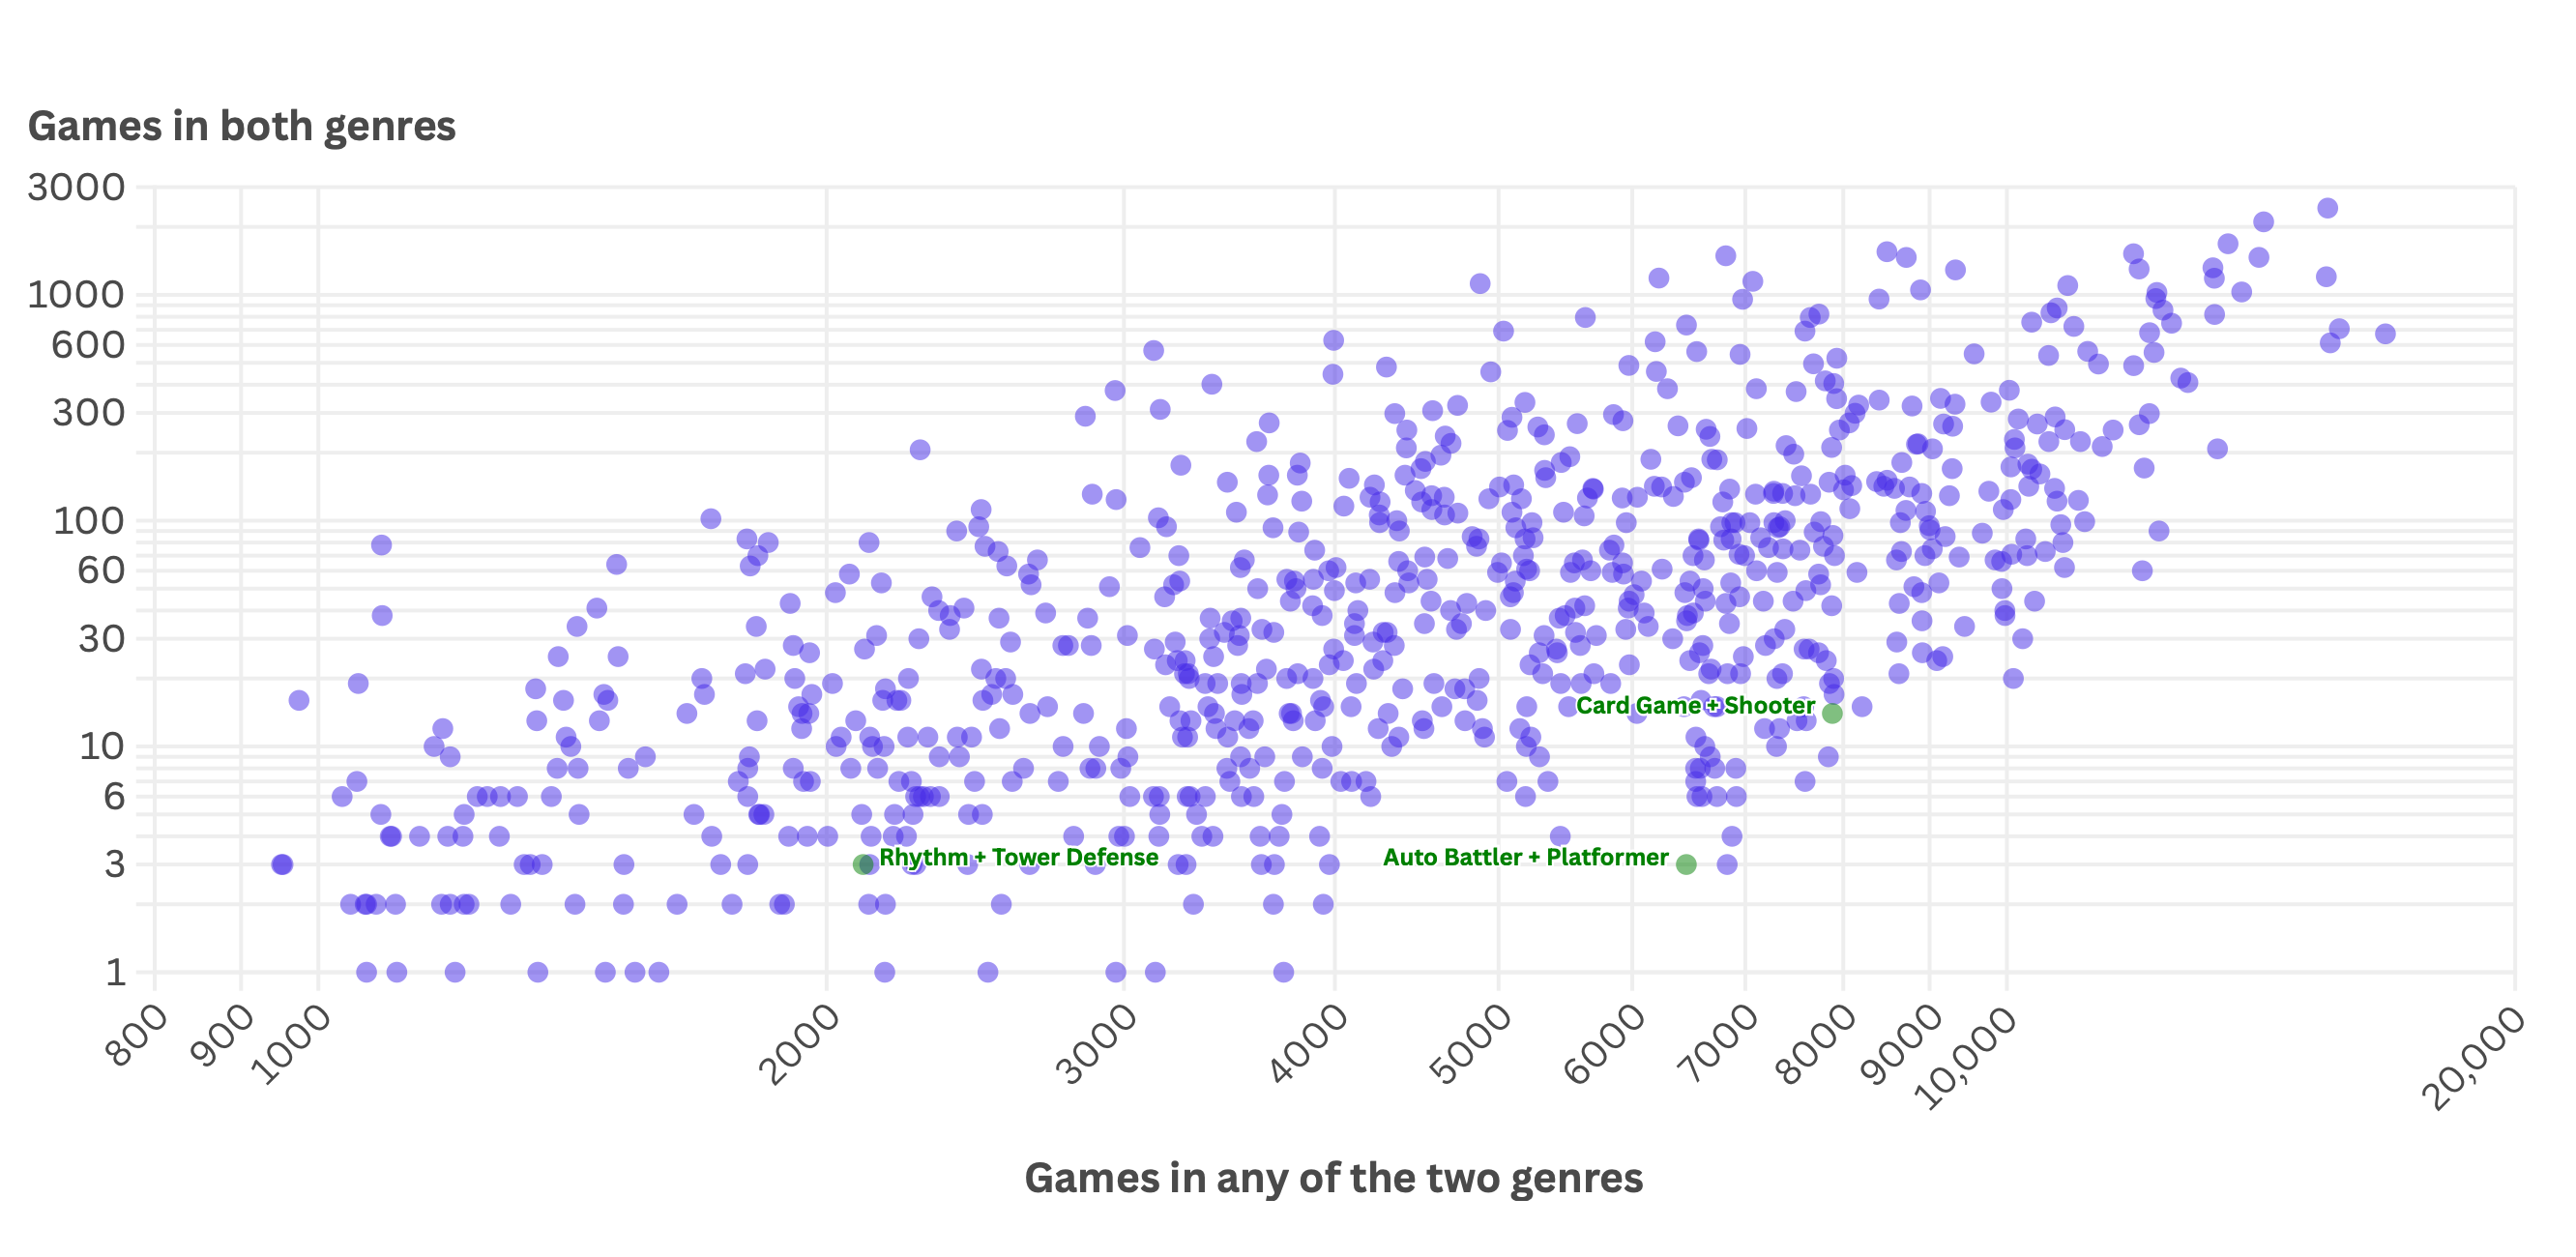
\includegraphics[width=\textwidth]{images/genre-pairs.png}
    \caption{Most frequent genre pairs}
    \label{figure:genre-pairs}
\end{figure}



\section{Game engines}

This thesis will include the development of a game prototype, and to reduce development time, a game engine will be used. There are many freely available game engines on the market at the time this thesis is being written, so to pick one, a short comparison needs to be made.

But first of all, what is a game engine? To answer this question, it would be a good idea to look back at the very first game engine. Doom Engine was developed for Doom (1993) by id Software, it was the first of its kind \cite{gregory2018gameEngineArchitecture}, the very first piece of software that had its components well-defined and separated, allowing developers to make different games with minimal modifications made to the game engine itself. Soon many major game development studios started to develop their own game engines, while licensing other's already working engines started to become a norm.

Developers today can also choose to use free-to-use game engines such as Unreal Engine \cite{unrealEngine} or Unity \cite{unity}. These engines are usually for general purposes, meaning that they include a handful of features that make it possible to develop any kind of video game with them, with the side-effect of being hard to learn on a professional level. Additionally, they are not entirely free, as there is usually a limit above which developers have to start paying a share of their total revenue to the engine. 

There are more compact alternatives, such as Godot\cite{godot} or LÖVE\cite{love2d}, which are completely free and open-source, meaning that developers can actively contribute to their code base to implement new features. However, they often lack features found in more robust engines.



\section{Game development} \label{Section:GameDevelopment}

Creating video games is a combination of several professions. It includes programming, game design, asset creation such as sprites, 3D models, music and sound effects, and even marketing. Dedicated tools can be used for each of these areas; some of them are discussed in Axel Ljungdahl's master's thesis \cite{ljungdahl2020individual} on individual game development. Axel's work is considered extremely valuable regarding this thesis, as it provides important tips and guidelines for how a game prototype should be developed individually, using only affordable tools.

For programming, code editors, or IDEs (Integrated Development Environments) can be used to help with coding syntax, formatting, and debugging, as well as code completion. Popular options include Visual Studio\cite{visualStudio}, Visual Studio Code\cite{visualStudioCode} and the JetBrains\cite{jetBrains} suite. Some game engines, such as Godot, even have their own integrated code editors. \cite{ljungdahl2020individual}

For creating graphical assets, like sprites or textures, one can choose between raster graphics, storing images as a grid of rectangular pixels, and vector graphics, storing images as mathematical models that can be scaled without using detail. Respectively, free tools such as GIMP \cite{gimp} and Figma \cite{figma} can be used for these approaches. If the game is three-dimensional, it usually requires 3D model assets, which can be created using Blender\cite{blender}. \cite{ljungdahl2020individual}

Music and sound effects can be created with free tools such as LLMS. Existing audio files can be edited using Audacity. Audio can also be recorded using a regular microphone found inside an average smartphone or laptop. Some games, like Samorost 3\cite{samorost3_2016}, use sound effects produced solely by mouth and real instruments.
\chapter{Methodology} \label{Chapter:Methodology}

This chapter describes the core problem and how this research plans to find answers to it.

% TODO: Create a separate game testing section



\section{Approach}

\textbf{Planning:} To find answers to RQ1, the thesis will begin with a short research and experimentation where genre combinations - that currently do not exist - will be explored and analyzed to determine whether they could function well together. To help with this research, Steam's video game database will be used, as it contains most modern video games and their necessary details. As a result of this part, a genre combination will be chosen with which the thesis can continue to its second part.

\textbf{Implementation:} To answer RQ2, the project will involve the design and iterative implementation of a game prototype that combines all the chosen game genres from Planning and their corresponding elements and game design patterns. 

During the project, between iterative cycles, the game prototype will be regularly tested on small player groups to gain instant feedback that could help the development stay on track.

At the end of the project, a formal game testing session will be conducted that will include presenting the game prototype to potential players and letting them play with it for a short time while being guided and supervised. At the end of the session, using a feedback form and verbal questions\cite{björk2015Interviews}, anonymous data will be collected that will show how the combined gameplay design patterns work together and what the players think of their experience. Additionally, the game will be internally evaluated using the extended version of the GameFlow model\cite{sweetser2017gameflow}.

Finally, a data analysis will be carried out on the feedback collected during the tests. This involves data collected from surveys, but also statistical data from the game itself that can be visualized using various methods\cite{björk2015DataVisualization}. 

Furthermore, during the thesis, regular meetings will be conducted with the project supervisor Natasha Mangan to discuss progress, deal with any problems at hand and plan the next steps.



\section{Tools}

To create the game prototype, preferably an existing game engine is used. As discussed in section \ref{Section:GameDevelopment}, there are several free-to-use game engines available, such as Unity, Unreal Engine, and Godot, just to name some of the largest. There are many tutorials, guides, and documentation available online for all three game engines. For this thesis, Godot will be used, because it is completely free, easy to learn, lightweight, and user-friendly, and it packs the necessary features for the intended game prototype.

Godot uses its own scripting language called GDScript, which is close to Python. However, in this thesis, Godot Mono will be used, which works with C\# instead, a much more widely used language.

To keep the code organized and secure, GitHub, a Git version tracking system, will be used. This way changes in the code can be tracked, and if anything goes wrong, it is possible to revert back to a previous version.



\section{Time plan}

The table below contains all the planned deadlines. Although this is a 30-credit master's thesis project, the time span is longer than the course schedule would suggest, because the work was started earlier.

\begin{center}
    \begin{tabular}{ l l l l }
        \textbf{Task}                   & \textbf{Start} & \textbf{End} & \textbf{Length} \\
        Detailed literature review      & December 1     & January  31  & 9 weeks         \\
        Exploring genre combinations    & January 1      & January 31   & 4 weeks         \\
        Developing the game prototype   & January 15     & April 1      & 10 weeks        \\
        Development testing             & February 1     & April 1      & 8 weeks         \\
        Game testing                    & April 1        & April 15     & 2 weeks         \\
        Reacting to feedback            & April 15       & April 26     & 2 weeks         \\
        Finishing up the Final Report   & April 29       & May 31       & 5 weeks         \\
    \end{tabular}
\end{center}



\section{Ethical considerations}

Anonymous feedback data will be collected during playtests. All playtesters will be informed about this in advance. Participation in the playtests will be voluntary and the participants can opt out at any time if they do not want to continue the playtest.

% Accessibility

Player accessibility must also be taken into consideration. This means using a color palette that can be easily distinguished by players with color blindness, supporting multiple controller types, and preferably re-mapping buttons. However, this thesis can focus only on so many things. Paying attention to every small detail, including accessibility, is not the top priority right now, as the main goal is to check whether the new game type works or not. If it does work, then the game can be extended with various accessibility features in the future.

\chapter{Planning} \label{Chapter:Planning}


This chapter discusses the process of selecting a genre combination to work with, and then explores ideas for possible game mechanics.


\section{Coming up with a genre combination}

This chapter will explain the process behind finding an answer to the first research question, which is "\researchQuestionOne".

Before real work on RQ1 started, during a few brainstorming sessions, a few ideas for genre combinations that felt like they were still unexplored had already been written down to check out later. The most promising among these was the "Extraction Deckbuilder", which is a combination of the "Extraction Shooter" - without the shooter aspect - and "Deckbuilding" concepts. Extraction on its own does not exist as a separate tag on Steam yet. This mix proved to be unique after conducting the following research:

After reviewing the data set discussed in chaper \ref{Chapter:Theory} and going through the less popular tags while filtering out those that do not represent a genre or sub-genre, still a lot of tags remained. There were 195 tags that appeared less than 1000 times in total. For comparison, the most used tag, "Singleplayer", appeared 72120 times. But we could go even lower, as there were 38 tags with which less than a hundred games were tagged. To limit the number of genre combinations to choose from, it seemed ideal to include at least one tag that has such a low occurrence. Most tags with low occurrence do not indicate genres, but rather specific game elements that the game includes, like "Fox", "Birds", "Dice", "Elf", and so on. Coincidentally, "Extraction Shooter" is one of the least used tags, the 33rd in the list counting from the back, with an occurrence of 84. Interestingly, at the time of writing, the number of games tagged with "Extraction Shooter" has already grown to 155, which is an 85\% increase compared to the data set, indicating that it is a trending tag (the occurrence of "Singleplayer" has only increased by 42\%).

Thus, using Extraction Shooter as a starting point is a good idea, and luckily when combining it with the Deckbuilding tag, there is not a single game in the data set that matches this combination. There is, however, one on Steam called Echo Chambers, but it does not have a release date yet, and based on its description and screenshots it severely differs from the type of game this thesis aims to explore. Therefore, the combination of extraction and deck-building mechanics can be considered a truly new mix.



\section{Defining Extraction Deckbuilder}

To better understand what exactly the term Extraction Builder means, each genre of which it consists of will be defined using definitions of gameplay design patterns \cite{gameplayDesignPatterns}.



\subsection{Deckbuilding}

This genre works with collecting and playing cards and deck management, similar to some board games like Century: Spice Road. Players can acquire cards that they add to their collection, from which they assemble decks to play with. The genre does not define the rules that imply exactly how the cards work and interact with each other, they are unique to each game. Some, like Balatro \cite{balatro2024}, are based on traditional playing cards, while others like Hearthstone \cite{hearthstone2014} or Gwent \cite{gwent2018} use their own set of cards. It is quite common in deckbuilders to have the ability to alter some card properties. In Balatro, players can add special abilities to cards, and even modify their suite or value. Some cards in Hearthstone modify their effects based on which cards the player has previously played, holds in their hands, or has in their deck. 

The closest genre from Mark J. P, Wolf's taxonomy\cite{wolf2002genre} is Card Games, while Strategy from Apperley's\cite{apperley2006genre} more ambiguous categories, and Games of Chance in Crawford's earlier list\cite{crawford1984art}.

The gameplay design patterns used in deckbuilders are the following:

\begin{itemize}
    \item \textbf{Cards}: the main \textbf{Resource}, with unique \textbf{Abilities} or some other game-altering effects.
    \item \textbf{Card building}: the modification of cards in various ways. Although not all deckbuilders utilize this pattern, it can be observed in Hearthstone\cite{hearthstone2014} and Balatro\cite{balatro2024}.
    \item \textbf{Decks}: a collection of cards that through shuffling, introduces the \textbf{Randomness} and \textbf{Luck} patterns.
    \item \textbf{Deck Building}: putting newly acquired cards in the player's deck for it to be drawn later. The core gameplay pattern of deckbuilders.
\end{itemize}



\subsection{Extraction Shooter}

This type of game is a recent alteration of the Tactical Shooter genre. Tactical Shooters, and Shooters in general, focus on using firearms as the main tool for destroying enemies or other players. One of the most popular Shooter sub-genres is FPS (First Person Shooter), where players control the game from their character's point of view. The Extraction Shooter genre first appeared in Escape from Tarkov\cite{escapeFromTarkov2017} in 2017. This kind of game is usually played in iterations called runs and features an open world that the player enters with some loot they have gathered in previous runs. During a run, the player has to explore and collect loot while fending off other players or NPCs (non-playable characters). At the end of a run, they have to reach an extraction point where they can safely leave the match with all the collected loot, adding it to their inventory outside of the match. However, if the player dies during a run, all the loot that they have collected, as well as the equipment they have brought in, will be lost forever. However, there are usually some twists, such as a safe pocket that keeps its content upon death. This type of game falls under the Combat Games category in Crawford's list\cite{crawford1984art}, Action in Apperley's, and Shoot 'Em Up in Wolf's taxonomy (while also borrowing elements from the Collecting genre). Interestingly, Extraction Shooters do not fit Wolf's Escape genre, as it does not allow the player to fight back.



\subsection{Extraction}

The term "Extraction" has not been used officially as a genre on its own yet, it is a made-up genre for this thesis only. To put it simply, it contains every game element Extraction Shooter does, except those related to the Shooter part, making it a more general category. It could be combined with other major genres, like Platformer or Strategy, but in this thesis, it will be mixed with Deckbuilding. 

The definition of extraction games is the following: 

\textit{Run-based games where players collect resources and must transport them to extraction points to retain them.}

Furthermore, players manage two inventories: an inner inventory used during runs and an outer inventory for permanent progression. Players can transfer loot between inventories outside runs. A run ends either by reaching an extraction point or by dying, which results in the permanent loss of loot in the inner inventory.

There are a few existing video games that fit into the extraction category, but are not extraction shooters. Deep Rock Galactic\cite{deepRockGalactic2018} for example, while containing some shooter elements, focuses more on collecting loot by mining and safely returning it to the extraction point. In lethal Company\cite{lethalCompany2023} players have to explore a procedurally generated facility, safely extracting items, while surviving against enemies, without a serious focus on combat. Even Soulslike games can be considered closely related to extraction games, where bonfires serve as extraction points and the soul is the loot, but the loot is not lost permanently if the player manages to retrieve it before dying for a second time. However, while, for example, Dome Keeper\cite{domeKeeper2022} definitely contains some extraction elements, it completely lacks the option of permanent loss of loot.

The core gameplay design patterns include the following:

\begin{itemize}
    \item \textbf{Loot}: The collectible valuables that need to be extracted. Usually some kind of \textbf{Resource}, \textbf{Equipment} or currency.
    \item \textbf{Inventories}: The storage in which the player keeps the collected loot.
    \item \textbf{Rescue}: The closest pattern to extraction, rescuing someone or something (loot) that is otherwise not free to move by its own will.
    \item \textbf{Enemies}: NPCs that are trying to stop the player from extracting loot, usually by attempting to kill them.
    \item \textbf{Replayability}: Due to the run-based nature of extraction games, they are highly replayable, and each run usually differs from the last.
    \item \textbf{Death Consequences}: Dying results in the collected loot being lost.
\end{itemize}



\subsection{Mixing Deckbuilding with Extraction}

The resources in extraction games do not have a specific type, however, since Deckbuilders already work with cards, which can be considered a resource, it makes sense to use cards as the obtainable loot in Extraction Deckbuilders. Card loots become even more interesting with the fact that cards are the key gameplay elements of Decbuilders, so gaining new cards can drastically change the gameplay while the run is in progress by allowing the player to immediately put the newly collected cards in use. On the other hand, making such a vital game element permanently losable is a risky move since players can easily get frustrated. But keep in mind that this is exactly what Extraction Shooters do, just instead of cards, those games have weapons and gear as the key resource. To allow the player to secure at least a small portion of the gathered loot, some options need to be provided, like the already mentioned safe pocket, or a system that in exchange for some in-game currency, ensures that an item will be kept if the player dies.

In order to make an extraction game, the player needs to extract loot from somewhere. In general, this 'somewhere' could be a large open-world map similar to Tarkov\cite{escapeFromTarkov2017}, but for this thesis that would set the scope extremely high. A more reasonable option is to use an abstract 2D grid-like world that can still be large, but it is much easier to maintain due to its simplicity. To achieve the feel of a large-scale map, a procedural generation algorithm\cite{van2013procedural} could be used to dynamically create the map as the player progresses. To keep things contained and manageable, the algorithm could place predesigned rooms next to each other, connecting them with doors, just like in Enter the Gungeon\cite{enterTheGungeon2016} or The Binding of Isaac\cite{theBindingOfIsaacRebirth2014}, greatly saving development time.

In Extraction Deckbuilders, the gameplay design patterns of Deckbuilders and Extraction games get mixed too, resulting in the following list:

\begin{itemize}
    \item \textbf{Cards} become the \textbf{Loot} and \textbf{Resource}.
    \item \textbf{Inventories} become \textbf{Decks}.
\end{itemize}



\subsection{Further ideas}

Apart from the essential game elements of Extraction Deckbuilders, a currency system could be used in the upcoming game prototype to make room for some permanent progression in between runs. The currency could be a type of resource that can be spent on upgrades such as the safe pocket, and is always kept (at least partially), regardless of whether the player completed the run successfully. Otherwise, if the player lost a run and did not have any means to keep part of the loot and they would also lose the currency, they might lose the motivation to continue.

Using cards for as many actions as possible could be another interesting twist. This would include movement, opening chests or doors, picking up items, etc. If the player cannot play a movement card for any reason, they are simply unable to move. However, this rule could greatly limit the player and might turn out to be annoying, so some basic actions should not be tied to playing the right cards. One way of dealing with this is to use multiple hands and decks, one for each category of action: Movement, Combat, and Interaction. Each deck could have their own cards and rule sets, for example the Movement deck can not be depleted, while the Combat deck needs a rest to reshuffle, and the cards from the Interaction deck are permanently discarded upon use. However, it should be kept in mind that multiple decks might easily multiply the complexity of the game, a scenario which, in the case of this thesis, should be avoided.

Cards could be played relatively free, as in Balatro\cite{balatro2024} or Gwent\cite{gwent2018}, or for a specific cost, usually called mana, like in Hearthstone\cite{hearthstone2014} or Marvel Snap\cite{marvelSnap2022}. For Extraction Deckbuilder, the use of mana is a better fit because the game prototype will likely include a turn-based combat system, and mana is perfect for limiting the number of actions the player can take per turn. So a system needs to be implemented that determines how much mana the player has each turn, as well as how much mana each card costs.

The most important type of card will be combat cards, as fighting enemies is the main way to get loot in many games. For an engaging combat system, there should be a variety of actions that a player can take during a fight. These could include swinging a sword, holding a shield, casting a spell, drinking potions, and maneuvering around the enemy. Furthermore, the player should have basic stats such as health, armor, and attack strength, and some more complex ones such as accuracy, critical strike chance, and dodge chance. Stat values could be altered by various factors including their initial value, modified by equipment, cast spells, used potions, and other buffs and debuffs.



\section{Prioritization methods}

Developing software in general requires serious planning and task prioritization to ensure that available resources and time are properly used. Doing so increases the likelihood of the project being finished in time and that its core components are developed first.



\subsection{Moscow prioritization} \label{section:Moscow}

The tasks are divided into four categories using the Moscow prioritization method. Each category indicates the importance of its tasks. Tasks in the \textbf{Must have} category need to be implemented for the game to be considered finished. The \textbf{Should have} category contains tasks that are intended to be part of the finished product, but are not essential. In \textbf{Should have}, the likelihood that the tasks are included is low, they would add to the experience but are far from necessary. And finally, \textbf{Won't have} is for the tasks that are no way to be implemented, at least for this iteration of the project.

The following is a list of the most important features that come or do not come with the prototype, categorized using the Moscow method.

\subsubsection{Must have}

\begin{itemize}
    \item \textbf{Game world}: A set of 2D tiles representing a top-down world where the player and other game objects can exist and perform actions. Contains the extraction locations, too.
    \item \textbf{Cards}: Collectible cards with abilities and other properties such as cost. Different cards can be played differently; some will require a target location or enemy to be picked in the game world, while others will be playable regardless of a target. 
    \item \textbf{Set of rules}: Rules that dictate how the game works, when the player draws cards, how the cards interact, and how enemies behave.
    \item \textbf{Playable character}: The character that the player controls in the game world.
    \item \textbf{Enemies}: Non-playable characters with unique behaviors, trying to kill the player, controlled by a simple algorithm.
    \item \textbf{Inventory or Deck}: Some way of storing and organizing cards. An outer and inner inventory are needed.
    \item \textbf{Combat system}: Some sort of logic for the player to damage enemies and for enemies to damage the player.
\end{itemize}

\subsubsection{Should have}

\begin{itemize}
    \item \textbf{Menu}: The first thing players see when launching the game should be a main menu, where they can enter the game world, adjust some settings, and exit.
    \item \textbf{Sprites}: 2D image files to represent game objects. Makes the game more pretty, but does not add functionality.
    \item \textbf{User interface}: Some basic way to show the stats of the player and the enemies they are currently fighting. 
    \item \textbf{Fog of war}: The entire game world should not be shown to the player initially. Instead, it should be revealed as they move around.
    \item \textbf{More interactable objects}: Doors, chests, and other things that the player can interact with. Extraction locations are one such object, and unlike the others, it is a must-have.
\end{itemize}

\subsubsection{Could have}

\begin{itemize}
    \item \textbf{Sound effects}: Most interactions should have their own sound. Improve immersion, give audio feedback to actions, and make it easier to distinguish between events.
    \item \textbf{Status effects}: Additional game mechanics seen in many games, would include poison, fire, frost, etc. They would be applied to enemies using special cards, and the player could also receive these effects from enemies. Status effects could interact with each other.
    \item \textbf{Large variety}: An increased variety of enemies, cards, and loot. Would improve replayability, but it is not necessary to showcase the novel game mechanics.
    \item \textbf{Minimap}: A miniature representation of the game world to aid player coordination.
    \item \textbf{Procedurally generated world}: Generating the world on the go is a great way to make it feel large-scale. However, it would most likely require too much effort and would not fit the needs of the thesis.
    \item \textbf{Animations}: Sprites, some text, and the movement of game objects could be animated if time allows.
    \item \textbf{Save}: The genre is heavily based on long-term progression; therefore, the game should save and load the game files. However, implementing it might not be necessary to test the core mechanics of the game during a short testing session.
\end{itemize}

\subsubsection{Won't have}

\begin{itemize}
    \item \textbf{Performance optimizations}: This would include dynamic loading of the game world, enemies, objects, and items based on the position of the player. It would only be necessary if scalability were a key goal. However, for the prototype, it is negligible. Instead, every game object will be loaded and handled together.
    \item \textbf{Tutorial}: A shorter version of the main gameplay loop with explanations. It would require implementing features that could be told verbally for game testers.
    \item \textbf{Music}: While it would greatly improve immersion, for the game prototype it is unnecessary.
    \item \textbf{Story}: To show how the game mechanics work, a story is not required.
    \item \textbf{Key mapping}: An accessibility setting that would allow the player to freely change the keyboard layout.
    \item \textbf{Multi resolution support}: The game will be only designed for the standard 16:9 aspect ratio, which usually means 1920 by 1080 screen resolution.
    \item \textbf{Cross platform support}: The target platform will be Windows. Other platforms will not be supported at this time.
    \item \textbf{Achievements}: This would be a nice way to motivate players to explore every corner of the game. However, implementing them takes time and should be omitted from the prototype.
    \item \textbf{Localization}: The game will be developed only in English.
\end{itemize}



\section{Concept} \label{section:concept}

The initial design question before starting the development of the prototype is what kind of game is the best to test the mix of the extraction and deck-builder genres. Extraction shooter games are usually First Person Shooter games that use 3D graphics, while most card games are 2D with a top-down view. After careful consideration, I chose a top-down approach with a grid-based 2D world to make development as easy as possible. Using 2D removes the need for 3D assets that tend to be more tedious to work with and also makes it easy to implement the game logic. 

The open world where each run takes place is a procedurally generated dungeon filled with rooms and corridors connecting them. Each room can contain enemies, chests, and extraction points. To make the game 

Although the main progression factor in extraction games comes from the collected and extracted loot, some permanent progression between runs (meta progression) is also crucial. The exact method chosen for this initially was meant to be the introduction of card types that can be spent on player stat upgrades (such as max health boost, increased hand size, and extended vision), similarly to how players can spend gold in Vampire Survivors to unlock permanent bonuses. However, this type of progression does not fit the deck-builder theme of the game (since spendable cards are really just a currency in disguise). Instead, the chosen meta-progression method became card upgrades: Three identical cards can be combined into a more powerful variant. Upgraded cards can also be upgraded further, up to a set limit.

To prevent players from losing everything when they die during a run, Escape from Tarkov uses two mechanics: safe pouches whose contents can be recovered, and insurance, which can be applied to any item in the player's inventory for a price. I will use the latter approach, but instead of putting a price tag on this feature (I want to prevent introducing a currency just for this purpose), I want to make insured cards extremely rare. Every card dropped from slain enemies and opened chests will have a small chance of being insured. Although this technically makes it possible for the player eventually to enter a run with only protected cards in their deck, the cards collected during the run can still be lost from the inventory.

For the game to have an ending, there will be a final boss that the player must defeat to finish the game. Exactly one boss will be generated inside each dungeon. Although this makes it possible to encounter it on the first run, it will be so powerful that the player has virtually no chance of defeating it early on.
\chapter{Implementation} \label{Chapter:Implementation}

\section{Used software}

I started working on the prototype as soon as the initial designs and concepts have been written down. GitHub Projects\cite{gitHub} was used as a Kanban board to keep track of the tasks defined in \ref{section:Moscow}. The development was not split into multiple sprints, but it was rather following the waterfall method with the addition of continuous adaptation to changing requirements.

The latest version of Godot .NET (which at the time of starting the project was 4.3) was chosen as the game engine, thus the game was written in C\#. Rider, an IDE (Integrated Development Environment) made by JetBrains exclusively for .NET, was used as an external code editor. 

Three different software products were tried and used for the graphic assets. The most frequently used was ProCreate running on an iPad Pro 2020, which was perfect for pixelart as it supports importing and creating custom pixel brushes. On desktop, GIMP and Affinity Photo were used simultaneously.

\section{General process}

First, the core gameplay was implemented, including the grid-based world and the movement system. I used Godot's built-in TileMapLayer class to display multiple layers of sprites: ground, decoration (grass and pebbles), wall, object (things the player can interact with, like an extraction point), and enemy layers. This allowed for overlapping tiles (such as an enemy standing on a decorated ground tile). Although TileMapLayers were easy to use for quick level design within the editor, they did have some limitations. For example, I wanted to animate the enemy movement by interpolating between its old and new position; however, tile map layers cannot display tiles between grid cells. Instead, I had to switch to using regular Sprite2D nodes for each enemy. To keep the comfort provided by using tile map layers, I made a method that populates the game scene with enemy packed scenes based on the enemy layer's cell data: wherever I use a certain tile inside the layer, the method will place an enemy corresponding to that tile's position and sprite inside the node tree. I did the same with objects and the player.

\subsection{Turn-based combat}

Initially the game was intended to be turn based, and would implement a simplified version of the combat system Baldur's Gate 3 uses. This would have meant that enemies would enter a combat state whenever they detect the presence of the player by either noticing them or receiving damage or a status effect from them. Then, based on a defined turn order and each character's own energy points, the player and enemies would take turns in which they can move and use spells, until their energy is depleted. At the beginning of each turn, energy would be replenished. 

An initial version of this system was successfully implemented in an early version of the prototype; however, enemy turns occurred in an instant, without a clear visual representation of each individual action, which made it extremely hard to understand what actually happened between the player's two turns.
To make enemy turns visually appealing and easy-to-follow, I wanted to add small delays between each action they take, for example, they would wait for half a second before every step they take. However, in order not to freeze the whole game while enemy turns last, their animations needed to run on separate threads using asynchronous programming, which added so much unnecessary complexity to the logic of the game, resulting in numerous bugs that were hard to debug due to their multithreaded nature.

Ultimately, for the sake of simplicity, I decided to remove the turn-based combat system in its former state and proceed with a much simpler approach, inspired by the Crypt of the Necrodancer\cite{necrodancer2015}, a 2D top-down rhythm dungeon crawler. Practically, turns got reduced down to a bare minimum: Each player action (movement, interaction, playing or discarding a card) is considered a whole turn, and thus performing one results in all enemies taking a turn as well. To match the player's reduced flexibility in their turn, the complexity of the enemy logic was also minimized in the same fashion. Although previously enemies had an energy bar, allowing them to take a few steps on their turn, with the new system in place, most of them only step one every other turn.



\section{Cards}

The most important part of the prototype was to develop a card system with a set of rules. Cards are the only resource in the game, they can be collected during runs and due to the extraction genre, they can also be lost when the player dies, if left unprotected.

In the final design, cards were separated into three containers: the deck contains cards that are in use during a run, the inventory is where the picked up cards go, and the stash is the safe storage where cards remain even after the player dies. Generally, cards cannot be transferred between the three containers, except at home or near a bonfire.

The cards in the deck are divided into three groups, similarly to board games that utilize playing cards.

\begin{enumerate}
  \item \textbf{Hand}: Cards with their face up, that the player is currently holding and is able to play or discard. 
  \item \textbf{Draw pile}: A stack of cards face-down from which the player draws after playing a card from the hand.
  \item \textbf{Discard pile}: Also a stack of cards facing down, where played or discarded cards go.
\end{enumerate}

There is a maximum hand size of 4 a deck size of 20, and no limit on the discard pile. However, the deck size initially was set to 30, which during internal tests felt too much, so it was reduced.



\subsection{Protection}

As mentioned in section \ref{section:concept}, cards can be protected to prevent such edge cases when the player loses all their cards, and thus can no longer do anything in the game. To assist in that and to give the player an opportunity to learn by failing, the starting cards are all protected.

Protection is indicated with a shield symbol in the upper left corner of a protected card. Protection can be carried over to upgraded cards if at least one of the used cards was protected, allowing the player to safely upgrade their starting deck.



\subsection{Single-use cards}

Some cards are considered \textit{utility} cards, most of which can be used once, and then they are lost forever. Such cards are marked with the keyword \textit{Unstable} in their descriptions. These cards, when played, do not go to the discard pile, even when protected; instead, they are lost forever. This feature prevents the exploitation of some powerful cards, such as golden keys, or the later discussed Escape card.



\subsection{Types}

The game started off with a minimal set of cards: one that heals the player (Heal), one that damages a single enemy (Smite), and one that damages over an area (Hurl). Over time, additional cards were added to enhance the experience. Some new cards were introduced simply to improve variety, like a card that damages enemies in an area, similarly to Hurl, but divides the damage equally between all the enemies hit. Other cards, like Rest and Shuffle were added for balancing reasons.



\subsubsection{Rest}

Rest is a card that shuffles the discard pile into the deck (except for already discarded Rest cards). This allows the player to last significantly longer between bonfire uses or extractions. The introduction of this card was also the main reason the deck size limit was reduced, as putting 15 Rest cards into the deck would allow the player to use the other 15 cards 15 times each (15 x 15 = 225 card uses in total) before needing a bonfire. With a size limit of 20, this mechanic can still be exploited, but the total card uses can only reach a maximum of 100. Additionally, Rest is one of the rarest cards in the game, found only sometimes in chests that require golden key cards, which is also hard to find. So, it is unlikely that the player will ever have 10 Rest cards in their deck.



\subsubsection{Shuffle}

Perhaps the most controversial card based on feedback from internal playtests, as it sometimes felt useless to the testers. It is similar to Rest, except that this time the hand gets shuffled into the deck, and then new cards are drawn. Its intended use is to prevent the player from discarding momentarily undesired cards from the hand, and instead put them away for later use. However, a valid criticism is that the current hand limit, which is four, is too small for this card to play a meaningful role in card management. If the hand capacity were to increase over time, as originally planned, Shuffle would receive more love.



\subsubsection{Guide}

When the final enemy, the Exterminator, was introduced, its location was entirely random, which turned out to be extremely frustrating when the player was actively trying to finish the game by defeating the boss. To resolve this issue, I added an additional, rare utility card called Guide that would mark the ground beneath the player, creating an arrow that points in the approximate direction of the boss, drastically reducing the time spent looking for it. Since this card only becomes useful in the late game, its low drop rate is acceptable early on, as players will likely have acquired at least one by the time they are strong enough to face the boss.



\subsubsection{Shield}

A more powerful alternative to Heal is Shield, which adds extra health points on top of the player's maximum allowed health. When the player receives damage, the shield points are first depleted and then the health.




\subsubsection{Escape}

The most rare card in the game, Escape allows the player to return home without a ladder, from anywhere. It was only added to have a card that truly feels like a legendary class loot. To prevent it from being too powerful though, it is unstable, so the player cannot reuse it for every run once they find one.



\subsection{Upgrades}

In the original plans, collecting cards was the only meta progression to be included in the prototype. Getting stronger would have been achieved by adding more and more cards to the deck until it is at full capacity, thus the player reaching their full potential. This quickly turned out not to be enough. Getting more and more of the same cards would just mean that the player can repeat the same tasks more during the run without actually feeling stronger.

Card upgrades were implemented as a solution. To upgrade one, three identical cards (the same type and upgrade level) are required at the workbench, a new object that can be found at home. Each card got a maximum upgrade level with predefined values (damage, range, healing amount) depending on level. However, some cards, such as keys and other utility cards, cannot be upgraded as they could not make any significant improvements.



\section{Procedural generation} \label{Section:ProceduralGeneration}

Initially, the game world was meant to be hand-made and quite small. However, I quickly realized that an extraction game needs a large, open map that allows exploration and long run times with sparse extraction points; otherwise, the game might become too easy and repetitive. To accomplish this, hand-crafting the entire map would have been a waste of time, and with fixed extraction point locations, the players could memorize the map and get in and out effortlessly. Instead, I decided to use a procedural dungeon generation algorithm following the method demonstrated by Bob Nystrom\cite{nystromProcedural2014}, extended with the placement of decorations, enemies, and objects. The algorithm consists of six stages:

\begin{enumerate}
  \item First, a number of randomly sized rectangular rooms are placed on the map. If a room overlaps with an already placed one, the new one is discarded. This process is repeated until the predetermined maximum number of attempts is reached.
  \item After the rooms are placed, a random maze generation algorithm is run that carves paths through all the areas that were left empty. As a result, the entire map is now filled with rooms or corridors.
  \item Then hallways are carved out of the walls between the rooms and the maze to make the whole map a single, connected region. Some hallways are generated with a locked door that requires a key to open, somewhat limiting the player's freedom.
  \item Dead ends are removed from the maze to improve exploration. This way every corridor leads to another room and the player will not feel frustrated or misled by paths that go nowhere.
  \item The ground and the walls are decorated based on their surroundings: the adequate wall sprite is selected from a tile map based on its eight neighboring tiles, and the ground is populated with foliage based on its position inside a room or corridor: denser foliage grows along the wall and inside corners.
  \item Finally, rooms are filled with extraction points, bonfires, chests, and enemies based on their size. One exit and one bonfire are always guaranteed, as there are at least two rooms generated exclusively for them. Similarly, a room is reserved for the player to spawn in. With the introduction of the Exterminator, the algorithm was extended with another signature room that is always reserved for the boss.
\end{enumerate}

In later stages of the development, randomized loot generation, along with randomized enemy levels and object density - according to the selected level of difficulty - was also added to the algorithm. With this update, different types of enemies started to drop different loot, defined by a list of probabilities. Additionally, with a higher level of difficulty came more and tougher enemies that yield more loot when defeated; however, extraction points and bonfires became more rare.

During internal tests, it was common that multiple bonfires or ladders were generated directly next to each other. Finding such a cluster was a huge advantage, as the player was able to reset their deck multiple times without any need for further exploration; but on the other hand, the rest of the map had a reduced amount of such objects, which resulted in some runs without finding any bonfire or extraction point. To solve this, a minimum distance between bonfires and ladders was introduced. If a newly generated bonfire was too close to any existing one, it was discarded. This process - similar to the process for rooms - was repeated until the maximum number of attempts was reached.

\subsection{Pretty walls}

In a tile-based game, walls are usually stored as a two-dimensional array of Boolean variables, where each true value means that the player cannot pass through the corresponding tile. There are multiple ways to illustrate this towards the player, the simplest and probably most boring solution being to use squares of uniform color for each wall tile. Alternatively, walls can be visualized by continuous lines along the connected edges of the wall tiles. However, a more advanced and elegant solution is to create a tilemap containing all possible wall shapes and then use the appropriate sprite for each wall tile.

\begin{figure}[h]
    \centering
    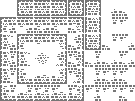
\includegraphics{images/walls.png} 
    \caption{All possible wall textures used in the prototype}
    \label{figure:walls}
\end{figure}

I decided to use a style that, in addition to visualizing the edge, also includes unique details inside the wall, depending on orientation, shape, and width. To achieve this style, there are exactly 48 possible wall shapes and orientations to choose from, shown in figure \ref{figure:walls}.

To retrieve the appropriate sprite from the tilemap, I first represented a tile's neighboring eight tiles as a bitmask, the greatest bit storing the value for the top-left neighbor, and following a reading order to store the others, the bottom-right neighbor being the last. Then I create a dictionary object, containing all the possible 256 in total bitmasks as keys, and the atlas coordinates (a two-dimensional vector representing a sprite's position inside the tileset) of their corresponding sprites. To make the process of filling up the dictionary slightly easier, I created patterns (similar to RegEx) consisting of eight nullable Booleans, describing the requirements for the bitmasks that correspond to the same sprite in the following way:

\begin{enumerate}
  \item If a bit must be 1 (wall), its value in the pattern is true
  \item If a bit must be 0 (empty), its value in the pattern is false
  \item If it does not matter whether a bit is 1 or 0, its value in the pattern is null
\end{enumerate}

Then I pass the patterns and the atlas coordinates of the desired sprite to a method that generates all possible bitmasks that match the pattern and adds them to the dictionary with the provided coordinates.

After the dungeon generation is finished, an additional pass is performed that is responsible for filling up the TileMapLayer with the adequate wall tiles, using the above-mentioned dictionary.

\subsection{Extraction points}

A defining part of extraction games are extraction points that players can use to leave the battlefield and return to a safe zone where they can manage the collected loot. In the prototype, ladders were used for such a purpose, which were randomly placed on the map. When the difficulty parameter was introduced, so was the minimum distance between the ladders, allowing them to be placed sparsely on higher difficulties.


\chapter{Results} \label{Chapter:Results}

For describing the finished prototype.

\section{Playtests}

\subsection{Showcases}

During the early stages of development, I conducted gameplay presentations, where I sat down and showed live gameplay to others and asked for feedback and ideas. These sessions were especially helpful, guiding me in the right direction regarding design decisions in gameplay. These presentations showed the game in a super early state, so the goal was simply to get an idea of whether the project was heading in the right direction.

\subsection{Early in-house tests}

When the game reached a state in which it was considered playable having a fully functional gameplay loop, I started conducting in-house tests with friends. I let them play the existing part of the game without any prior explanations and watched how they explored the controls and tasks. From time to time I added comments on a certain feature missing when the player was approaching its intended place (i.e., extraction points were already present in the generated map but were not functional). The first of these tests were using a version of the game with limited card and enemy variation, terrible balancing, and the complete lack of meaningful meta-progression. Since the game was far from its intended state, the true goal of these tests was only to gain more early feedback about whether the core concept of the game is functional and can be built upon. Most of the reactions I received were about the lack of variety in the game, which was naturally expected. Suggestions were made to add more content and variety to the dungeon generation method, but in general, everyone thought that the combination of the extraction and deck-builder genres was a unique and viable idea.

\subsection{Advanced in-house tests}

After responding to the feedback and finishing all the remaining tasks, a series of more serious tests was started, during which players were presented with a finished, feature-complete game. The test consisted of a complete playthrough of the game, as well as an extensive discussion afterwards, during which I took notes, guided by an early version of the feedback form used later in the public playtest. Three of these tests were conducted, with a gap of a few days between them that allowed the implementation of improvements and requested features.

During the first test, it became clear that the way the inventory and card upgrade menu was designed made it extremely slow and tedious to upgrade a large number of cards at once. In that version, the player had to first move all cards they were planning to upgrade from the inventory (or deck) to the stash by dragging them one by one from one container to the other. Furthermore, the cards were not sorted alphabetically or in any other way; their position in the list was determined by the order in which they were added to the container, so the player had to constantly search for the desired cards. At the workbench, they also needed to look through the whole list of cards placed in the stash to find the ones they wanted to upgrade, then drag them one by one to one of the upgrade slots, and then finally drag the upgraded version back to the stash container. Additionally, cards that could not be upgraded were also listed and could be dragged onto the upgrade area; only when all three upgrade slots were filled with cards would the game alert the player that the current card is already at its maximum level. Considering that most cards could be upgraded four times back then, to achieve the maximum upgrade for a single card, a total of 3 + 9 + 27 + 81 = 120 upgrade cycles were required, which is a ridiculous amount, especially if we take into account the time it takes to go through just a single cycle.

It was also pointed out that the game, especially the randomly generated maps that resulted from the procedural dungeon generation algorithm, felt boring and empty. As soon as the player had met all the enemies and found all the card types, there was nothing new or exciting to discover that would keep the player playing. The best way to solve the lack of this mystery factor would be a complete rework of the map generation method, with the introduction of biomes (distinct regions of the map) and secrets (rare rooms and enemies, areas locked behind special doors, etc.). However, all of these features would not fit the scope of this thesis.

The second test went much more smoothly, since most of the features requested from the first test were implemented by the time it was conducted, making the game much more enjoyable. All menus featured a sorted list of cards, and the cards could be dragged to the upgrade area from any container, as all of their contained cards were combined into a single list. The cards got an indicator in their top right corner showing which container they originate from, helping the player keep track of what cards they are using for the upgrade. However, the upgraded card variant was always put in the stash container, regardless of where its components originated. A good suggestion to solve this was made during the test: if at least one card originates from the deck, then the upgraded card should go to the deck instead. Similarly with the inventory: if at least one card originates from there and there are no cards from the deck, then the upgraded card goes to the inventory, otherwise the stash. This simple logic felt the most natural during testing, so it became the permanent solution. Additionally, even though the upgrade process has been dramatically sped up since the last test and the maximum level of cards was reduced to three, based on feedback, it still did not meet the expectations and was slow to use. However, making it even faster was no longer a high priority.

Since the first test, a new difficulty system has also been implemented that largely increased the feel of progression. Higher difficulty levels meant fewer extraction points, fewer bonfires, a higher number of enemies, and an even higher yield of loot from each of them.

Another requested feature was that the game should save occasionally. Since the game is a couple hours long, it would indeed be a good idea to implement saving to prevent loss of progression in case the tester cannot play the game for hours straight. However, saving should prevent players from escaping a deadly situation by simply closing and reopening the game and loading an earlier save. To accomplish this, the save file contained a flag about whether the last run started was formerly finished. When the game was launched, it checked for this flag, and if it was false, it treated the last run as if it was ended by player death, thus erasing all the unprotected cards from the deck and inventory.

Aside from additional balancing and detecting small bugs, the third and last test served as a confirmation that everything was working as intended and that the game could enter the public playtest state. 

\subsection{Public playtest}

After making sure that every part of the game was functional and thoroughly tested, I set up a project page on itch.io, created a feedback form using Google Forms, and advertised the game among university groups and friends. A deadline of one week counted from posting was set to conclude the test in time; however, this later was extended due to the surprisingly low number of downloads and form responses.

To make the test more accessible, testers were not required to complete a full playthrough of the game, as it would likely have taken multiple hours. Instead, they were asked to try to play the game as long as they could and then fill out the feedback form. During internal tests, the average time it takes to beat the game was estimated to be around two hours, but this result was achieved by continuously guiding the players when they felt stuck or did not understand a rule in the game.



\subsubsection{Hotfixes}

Three days after the original demo version was released, a quality-of-life feature was added to the workbench menu as the 1.1 hotfix patch, which made upgrading cards slightly faster. Instead of dragging cards from the list container over to the upgrade slots, they could simply click on a card to make it instantly jump to the first free slot. Similarly with the upgraded card: clicking on it puts it back into the list. This small enhancement made the upgrade process significantly faster, and thus likely reduced the total time it takes to beat the game, as it was shown during internal tests that card upgrades take up a considerable part of the gameplay loop.

Another correction was made in the 1.2 patch. Previously, the card sorting algorithm did not take into account whether a card was protected or not, and as a result, the order of protected and unprotected cards, which were otherwise identical, was undefined. This issue was caused due to a missing comparison between the protected flag of the card class. After the update, the protected cards were sorted ahead of others. Additionally, the previous patch was not thoroughly tested due to its quick release, so it shipped with a bug that could be exploited to duplicate cards using the workbench. This issue was also resolved.

Finally, a fix was implemented in the 1.3 version that solved a critical issue introduced also with the 1.1 patch. When the player were to click on a card in the hand during a run without starting to drag it, the game would enter an unresponsive state due to a wrongly set Boolean flag, and would stay that way until a card is properly played or discarded.



\subsubsection{Feedback}

\todo{Finish after playtest is concluded}
\chapter{Discussion} \label{Chapter:Discussion}



\section{Limitations}

This section lists some areas that were cut from the final prototype in order to reduce the scope and save time. Most of these features are planned to be implemented in future versions.


\subsection{State machines}

A popular approach to designing complex enemy behavior is to use state machines. Most games, such as Elden Ring\cite{eldenRing2022} and Hearthstone\cite{hearthstone2014}, use something close to state machines to keep track of the current state of every game object. State machines make it easier to implement different behaviors based on the state in which a game object is currently in. For example, a boss in Elden Ring\cite{eldenRing2022} usually has many repeating attack patterns that without a state machine would require tons of if statements, checking for the current player distance, what the previous attack was, or what phase the boss is in. However, with a state machine, different behaviors are well divided and do not rely on each other as the logic of state transitions is managed separately. This results in a more maintainable and scalable code in the long run.

This game could have also used such a system, but time constraints did not allow it to. Additionally, the extra complexity by implementing state machines was not necessary, since the logic of most enemies (except the Ranger and the Exterminator) consists only of these three states:

\begin{itemize}
  \item Idle (stand still, check if the player is in view)
  \item Follow player (while in view)
  \item If close enough, attack player
\end{itemize}



\subsection{Enemy intel}

In the early version of the prototype, cards that target an area or an enemy were not using any indicator as to where their casting range or damaging area were. These numbers were only shown in their description and nowhere else, so some playtesters were rightfully confused when they did not hit the enemy they were aiming at. As a quality of life improvement, colored area and range markers were implemented that are displayed when aiming with a selected card.

A similar feature was planned that would have shown where enemy attacks will land in the enemy's next turn, giving the player a clear warning about what tiles are considered dangerous. This would have also made it easier to understand how certain enemies work, as during the playtests the Ranger was especially pointed out to have confusing logic. However, due to time limitations, this idea was scrapped from the prototype, as it would also have required a complete rework of enemy behaviors to allow for a way to predict their next attack. Instead, players are left to discover each enemy's attack patterns.

A feature that would have allowed the player to inspect an enemy by clicking on it, gaining a detailed overview of its logic, stats, and drop rates, was also removed from the scope.



\subsection{Variety}

Having a large selection of cards is essential for deck-builder games. Collecting all the different cards can be a great motivator for players, making the game replayable. However, with great car variety comes a huge number of tasks: designing each card's logic, implementing, and then balancing it. To keep the scope of the prototype appropriate, the variety was classified as low priority.

Dungeon crawlers are also known to have numerous enemy types to keep traversing the dungeon exciting. For similar reasons, the enemy variety was also reduced.

The dungeon generator algorithm is also considerably simple, as it only generates rectangular rooms with a tight maze connecting them. There are no special rules for rooms with unique shapes, closed regions, or areas with a different style.

There were plans to extend the algorithm so that it would generate rooms without any entrance, making it only accessible using Teleport. Furthermore, rooms containing bonfires or ladders would have been more likely to be closed behind doors on higher difficulties, making the Wooden Key card viable in the late game.



\subsection{Tutorial}

Having a tutorial was ruled out during the process of writing down the concept for the game. However, back then the exact method used for the test was not yet selected. Later, it turned out that the testing will take place entirely online, and players would need to learn the rules of the game on their own. For that purpose, a short tutorial would have been the best option, but there was not enough time left to start working on a proper introductory level. The only feature resembling a tutorial that was implemented was an indicator that only shows up when the player first starts dragging a card from hand during a run, telling the player where to drag-and-drop a card to play or discard it.

As a replacement, a help panel, accessible from the pause menu, was included that describes the basic rules and concepts of the game with additional helpful tips. Furthermore, a text box was added to the main menu screen with information about the playtest and how to access the help menu. Most of this information was also included on the game's itch.io page.



\subsection{Accessibility}

As stated in section \ref{section:concept}, accessibility had a low priority throughout the project to save as much time as possible and instead shift the focus on making the combination of the genres work.
\chapter{Conclusion} \label{Chapter:Conclusion}

Draw the final conclusions and answer RQ2: \researchQuestionTwo

% Process and Execution OR Implementation
% Write about how I set up things, what didn't work, and progress, testing

% Final testing: what can it do, and why is it not good in something

% If the rq changes, talk about the reason for the change

% RESULTS
%% CREATED BY DAVID FRISK, 2016
\chapter{Results}
Describe your results. Use tables, diagrams etc. for illustration.

% CONCLUSION
%% CREATED BY DAVID FRISK, 2016
\chapter{Conclusion}

You may consider dividing this chapter into a discussion of the results and a summary. 

\section{Discussion}

\section{Conclusion}


% REFERENCES / BIBLIOGRAPHY
\cleardoublepage
\phantomsection % So hyperref does not link to the section above

\addcontentsline{toc}{chapter}{Bibliography}
\printbibliography

% APPENDICES
%\cleardoublepage
%\appendix
%\setcounter{page}{1}
%\pagenumbering{Roman}			% Capitalized Roman numbering starting from I (one)

%% CREATED BY DAVID FRISK, 2016
\chapter{Appendix 1}




\end{document}